\documentclass[onecolumn,10pt,cleanfoot]{asme2ej}

\usepackage{graphicx} %% for loading jpg figures
\usepackage{bm}
\usepackage{nicefrac}
\usepackage{mathtools}
\usepackage{amssymb}
\usepackage{amsmath}
\usepackage{parskip}
\usepackage{listings}
\usepackage{tablefootnote}
\usepackage{float}
\usepackage{xcolor}
\usepackage{xurl}
\usepackage{tikz}
\usepackage{caption}

\author{Grzegorz Kajda
    \affiliation{
	Bachelor Student, Robotics and Intelligent Systems\\ \\[-10pt]
	Department of Informatics The faculty of Mathematics and Natural Sciences\\ \\[-10pt]
    Email: grzegork@ifi.uio.no
    }
}


\begin{document}

\title{Simulating the Lipkin-Meshov-Glikov model on a classical computer}

\maketitle

\section{Abstract}

We present a comprehensive simulation of the simplified Hamiltonian of the Lipkin-Meshov-Glikov (LMG) model on a classical computer, employing the Variational Quantum Eigensolver (VQE) algorithm. Initially, we explore the outcomes arising from the application of diverse single qubit quantum gates to one qubit systems prepared in basis states. Subsequently, an entangler circuit is constructed, and one of the four bell pairs is prepared, to which we apply the Hadamard and CNOT gates. Utilizing our newfound grasp of the foundational principles governing quantum systems, we construct quantum circuits for generating ansatz states and methodically develop the VQE from ground up.

To assess the VQE's efficacy, we apply it to synthetic quantum systems representing single and two-particle systems, comparing its performance against numerical and analytical solvers. Transitioning to the Lipkin model, we leverage the properties of annihilation and creation operators to reformulate the Lipkin model's Hamiltonian first in terms of the quasi-spin operator and then Pauli operators. Employing this encoding scheme, we apply the VQE to systems with spin J=1 and 2, corresponding to Lipkin systems with two and four fermions, respectively. We compare the results against exact solutions obtained through standard diagonalization methods. This analysis provides valuable insights into the performance and accuracy of the VQE approach in tackling the Lipkin model's Hamiltonian.
	

\section{Introduction}
Since its emergence in the early 1900s, quantum mechanics has sparked fervent discussions among physicists, engaging luminaries of modern physics like Einstein, Dirac, Bohr, and many others. The discovery of the quantum realm profoundly reshaped our perspective and understanding of the world around us, unveiling a whole new realm of fundamental principles governing the very building blocks of the universe. With the advent of computer systems in the latter half of the 20th century, and the introduction of the quantum Turing machine in 1980, the field of quantum computing was born, ultimately leading to the construction of the first quantum computer in 1998. Recently, due to technological advances and discovery of new quantum algorithms, we have been granted to an extent, the capability of simulating simple many-body quantum models using classical computers.

An emerging research area in quantum computing focuses on the simulation of nuclear physics, leveraging the unique properties of quantum systems. Nuclear systems possess distinct characteristics that make them well-suited for exploration using quantum computers, providing insights into particle interactions. However, it is worth noting that quantum computers still face challenges, such as larger error rates compared to classical computers and vulnerability to noise, which can make working with them potentially difficult. Although the field of quantum computing is expanding rapidly, widespread accessibility remains limited, with companies like IBM offering only highly restricted access to their quantum technology. In light of these factors, we will employ a classical computer to simulate and analyze the simplified Lipkin-Meshkov-Glick model, showcasing the potential that quantum computing holds while acknowledging the current limitations in accessibility.

To facilitate our simulations, we will begin by constructing quantum circuits using single-qubit quantum gates. This approach will allow us to implement the Variational Quantum Eigensolver (VQE) algorithm effectively, enabling us to approximate the ground state energy of the Lipkin model for systems composed of two and four particles.

Apart from the introduction, this paper is organized into four sections. In Section Two, we will provide a comprehensive description of the theory and methods employed in this study. Following that, we will present our results, and finally, conclude with a summary of our findings.
 
 \section{\textbf{Section II: Theory and Method \\}}

 \subsection{Quantum gates}
The primary distinction between classical computers and their quantum counterparts lies in the nature of the data they process. In classical computing, the fundamental data unit is the binary digit, commonly known as a bit, which represents different voltage levels associated with low and high states. On the other hand, quantum computers utilize particles, such as atoms, as the information unitm leading to a fundamentally different approach to data handling. The unique properties of atoms and the underlying principles of quantum mechanics prevent us from treating them in the same manner as classical bits. For instance, in classical computing, logical gates like \textit{and}, \textit{or}, \textit{xor}, and \textit{nand} are commonly used for data processing, but these gates produce irreversible outcomes. However, on quantum computers, irreversible outcomes are generally not allowed, except in the case of measurement.

On a quantum computer, the fundamental data type used for storing information is the \textit{qubit}, which represents the digital manifestation of the wave function for a quantum particle. The principles of quantum mechanics dictate that the evolution of a quantum system can be mathematically described using unitary operators. This implies that the operations applied to quantum systems are inherently reversible. Consequently, at any given point in time, a quantum system can be fully characterized by a set of linear unitary operators. As a result, data processing on a quantum computer necessitates the use of reversible operators, enabling the "uncomputation" of the outcomes produced by quantum gates. The most basic of these operators are typically represented using 2x2 matrices. While these 2x2 operators quantum gates operate on individual qubits, by utilizing the Kronecker product (tensor product), we can in theory construct gates for quantum systems composed of arbitrary number of qubits. In practice we will often find ourselves restricted to at most 8 or 10 qubits before the computational overhead becomes too high.

The following are the basic quantum gates which we will utilize to contruct more complex gates and ciruits: 

\begin{enumerate}
	\item[\textbf{I}.] \textbf{Identity gate}
		\begin{equation*}
			I = \begin{pmatrix}
			1 & 0 \\
			0 & 1 \\
		\end{pmatrix}.
	\end{equation*}

	\item[\textbf{II.}] \textbf{Pauli-X gate}
		\begin{equation*}
			X = \begin{pmatrix}
			0 & 1 \\
			1 & 0 \\
		\end{pmatrix}.
	\end{equation*}

	\item[\textbf{III.}] \textbf{Pauli-Y gate}
		\begin{equation*}
			Y = \begin{pmatrix}
			0 & -i \\
			i & 0 \\
		\end{pmatrix}.
	\end{equation*}

	\item[\textbf{IV.}] \textbf{Pauli-Z gate}
		\begin{equation*}
			Z = \begin{pmatrix}
			1 & 0 \\
			0 & -1 \\
		\end{pmatrix}.
	\end{equation*}

	\item[\textbf{V.}] \textbf{Hadamard gate}
		\begin{equation*}
			H = \frac{1}{\sqrt{2}} \begin{pmatrix}
			1 & 1 \\
			1 & -1 \\
		\end{pmatrix}.
	\end{equation*}

	\item[\textbf{VI.}] \textbf{Phase gate}
		\begin{equation*}
			S = \begin{pmatrix}
			1 & 0 \\
			0 & i \\
		\end{pmatrix}.
	\end{equation*}

\end{enumerate}

\subsection{Lipkin-Meshkov-Glick model}
The Lipkin-Meshkov-Glick (LMG) model, often called Lipkin model, is a quantum model describing the collective beahvior of a large number of particles which was introduced in 1964 for the purpose of studying approximation methods used to solve many-body problems. Since its introuduction, it has become one of the standard benchmarks [Physical review C] for many-body methods in nuclear and particle physics. The model describes a system of N fermions (i.e. particles with half-integer spin values like electrons and quarks) which are distributed among two energy levels with quantum numbers $\sigma$ = ±1. The upper level has $2\sigma$ = +1 and energy $e_{1}$ = $e/2$, while the lower level has $2\sigma$ = -1 and energy $e_{2}$ = $e/2$. This can be visualized in the following way

\begin{figure}[H]
	\centering
	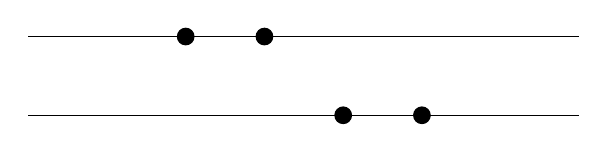
\begin{tikzpicture}
	  % Draw the parallel lines
	  \draw (0,0) -- (7,0);
	  \draw (0,1) -- (7,1);
	  
	  % Draw the small circles on the lines
	  \foreach \x in {2,3}
	  {
		\filldraw (\x,1) circle (3pt);

	  }
	  \foreach \x in {4,5}
	  {
		\filldraw (\x,0) circle (3pt);
	  }
	\end{tikzpicture}
	\caption{Figure showing the distrubution of four fermions among two energy levels}
\end{figure}

The figure depicts two horizontal lines representing the mentioned distinct energy levels, while the dots on the lines represent four fermions that in this case are evenly distributed between these levels. Each fermion in the figure corresponds to its own substate, characterized by quantum numbers $p = 1, 2, 3, 4$. It is important to note that in the figure, each particle occupies its own unique state. This behavior is typical of fermions, which obey the \textit{Pauli exclusion principle} [Basdevant, p. 348], meaning that two independent fermions cannot occupy the same state at exactly the same time.

Now the Lipkin model is described through its Hamiltonian given by 
\begin{equation}
\hat{H} = \hat{H}_{0} + \hat{H}_{1} + \hat{H}_{2}.
\end{equation}

where each of the the $\hat{H}_{i}$ can be written in terms of the creation and annihilation operators

\begin{equation}
\hat{H}_0 = \frac{1}{2}\varepsilon\sum_{\sigma,p}\sigma a_{\sigma,p}^{\dagger}a_{\sigma,p},
\end{equation}

\begin{equation}
\hat{H}_1 = \frac{1}{2}V\sum_{\sigma,p,p'} a_{\sigma,p}^{\dagger}a_{\sigma,p'}^{\dagger}a_{-\sigma,p'}a_{-\sigma,p},
\end{equation}

\begin{equation}
\hat{H}_2 = \frac{1}{2}W\sum_{\sigma,p,p'} a_{\sigma,p}^{\dagger}a_{-\sigma,p'}^{\dagger}a_{\sigma,p'}a_{-\sigma,p}.
\end{equation}

The role of creation and annihilation operators in a quantum mechanical many-body model is to highten and lower the number of particles in a given substate by one, respectively. For instance, applying an creation operator to the upper energy level of \textit{Fig.1} would increase the number of fermions by one in that energy level. A useful property of these operators allows us to use them to express the Hamiltonian of the Lipkin model in terms of the so-called \textit{quasi-spin operators} and \textit{number operator}. Defining he quasi-spin operators as 

\begin{equation}
\hat{J}_{+} = \sum_{p} a_{p+}^{\dagger}a_{p-},
\end{equation}

\begin{equation}
\hat{J}_{-} = \sum_{p} a_{p-}^{\dagger}a_{p+},
\end{equation}

\begin{equation}
\hat{J}_{z} = \frac{1}{2}\sum_{p\sigma} \sigma a_{p\sigma}^{\dagger}a_{p\sigma}, 
\end{equation}

\begin{equation}
\hat{J}^{2} = J_{+}J_{-} + J_{z}^{2} - J_{z}.
\end{equation}
















 


\end{document}


